\begin{appendix}
\chapter{Anexo: Discretización de las Ecuaciones del BOM}\label{AnexoA}
En este apartado se presenta la discretización de las Ecuaciones del BOM \ref{ec:aceite}, \ref{ec:gas}, \ref{ec:agua} que se presentan en la subsección \ref{subsec:BOM}. Recordando:
\begin{align*}
\text{aceite: }&\frac{\partial}{\partial t} \left[ \phi \left( \frac{S_{o}}{B_{o}} + \frac{R_{v} S_{g}}{B_{g}} \right) \right]
- \nabla \cdot \left( \frac{1}{B_{o}} \vec{u_{o}} + \frac{R_{v}}{B_{g}} \vec{u_{g}} \right) - \tilde{q}_{o}=0  \\
\text{gas: }&\frac{\partial}{\partial t} \left[ \phi \left( \frac{S_{g}}{B_{g}} + \frac{R_{s} S_{o}}{B_{o}} \right) \right]
- \nabla \cdot \left( \frac{1}{B_{g}} \vec{u_{g}} + \frac{R_{s}}{B_{o}} \vec{u_{o}} \right) - \tilde{q}_{g} = 0 \\
\text{agua: }&\frac{\partial}{\partial t} \left[\phi \left( \frac{S_{w}}{B_{w}} \right) \right] - \nabla \cdot \left( \frac{1}{B_{w}} \vec{u_{w}} \right) - \tilde{q}_{w} = 0 
\end{align*}
Primero, se integran las ecuaciones sobre un intervalo de tiempo $\left[t, t+\Delta t\right]$, y una celda de control $\Omega_{i}$. Se toma como ejemplo la ecuación de conservación para el aceite \ref{ec:aceite}. Las ecuaciones para el gas y agua (\ref{ec:gas}, \ref{ec:agua}) se discretizan de manera análoga.
\begin{align*}
	\int_{t}^{t+\Delta t}\int_{\Omega_{i}}\frac{\partial}{\partial t} \left[ \phi \left( \frac{S_{o}}{B_{o}} + \frac{R_{v} S_{g}}{B_{g}} \right) \right]dVdt
	- \int_{t}^{t+\Delta t}\int_{\Omega_{i}}\nabla \cdot \left( \frac{1}{B_{o}} \vec{u_{o}} + \frac{R_{v}}{B_{g}} \vec{u_{g}} \right)dVdt \\
	- \int_{t}^{t+\Delta t}\int_{\Omega_{i}}\tilde{q}_{o}dVdt=0 
\end{align*}
Luego, se desglosan las ecuaciones en sus términos acumulativos, de flujo, y de fuentes y sumideros, debido a que cada uno de estos términos requiere un tratamiento distinto.
\begin{align*}
\underbrace{\int_{t}^{t+\Delta t}\int_{\Omega_{i}}\frac{\partial}{\partial t} \left[ \phi \left( \frac{S_{o}}{B_{o}} + \frac{R_{v} S_{g}}{B_{g}} \right) \right]dVdt}_{\text{Término de acumulación}}
- \underbrace{\int_{t}^{t+\Delta t}\int_{\Omega_{i}}\nabla \cdot \left( \frac{1}{B_{o}} \vec{u_{o}} + \frac{R_{v}}{B_{g}} \vec{u_{g}} \right)dVdt}_\text{Término de flujo} \\
- \underbrace{\int_{t}^{t+\Delta t}\int_{\Omega_{i}}\tilde{q}_{o}dVdt}_{\text{Término de fuentes y sumideros}}=0 
\end{align*}
Empezando por el término acumulativo, se sigue que, por el teorema de Fubini que
\begin{align*}
	\int_{t}^{t+\Delta t}\left(\int_{\Omega_{i}}\frac{\partial}{\partial t} \left[ \phi \left( \frac{S_{o}}{B_{o}} + \frac{R_{v} S_{g}}{B_{g}} \right) \right]dV\right)dt = \int_{\Omega_{i}}\left(\int_{t}^{t+\Delta t}\frac{\partial}{\partial t} \left[ \phi \left( \frac{S_{o}}{B_{o}} + \frac{R_{v} S_{g}}{B_{g}} \right) \right]dt\right)dV 
\end{align*}
Por teorema fundamental del cálculo
\begin{align*}
 \int_{\Omega_{i}}\left(\int_{t}^{t+\Delta t}\frac{\partial}{\partial t} \left[ \phi \left( \frac{S_{o}}{B_{o}} + \frac{R_{v} S_{g}}{B_{g}} \right) \right]dt\right)dV = \int_{\Omega_{i}}\left[ \phi \left( \frac{S_{o}}{B_{o}} + \frac{R_{v} S_{g}}{B_{g}} \right) \right]^{t+\Delta t}_{t}dV
\end{align*}
Considerando el cambio de la acumulación en un intervalo de tiempo como una constante para una celda de control $\Omega_{i}$
\begin{align*}
	\int_{\Omega_{i}}\left[ \phi \left( \frac{S_{o}}{B_{o}} + \frac{R_{v} S_{g}}{B_{g}} \right) \right]^{t+\Delta t}_{t}dV = \left[ \phi_{i} \left( \frac{S_{o,i}}{B_{o,i}} + \frac{R_{v,i} S_{g,i}}{B_{g,i}} \right) \right]^{t+\Delta t}_{t}\int_{\Omega_{i}}dV \\= |\Omega_{i}|\left[ \phi_{i} \left( \frac{S_{o,i}}{B_{o,i}} + \frac{R_{v,i} S_{g,i}}{B_{g,i}} \right) \right]^{t+\Delta t}_{t}
\end{align*}
Donde $|\Omega_{i}|$ es el volumen para una celda $i$. Continuando con la discretización del término de flujo, se discretiza primero el tiempo usando un esquema \textbf{implícito}, luego
\begin{align*}
\int_{t}^{t+\Delta t}\int_{\Omega_{i}}\nabla \cdot \left( \frac{1}{B_{o}} \vec{u_{o}} + \frac{R_{v}}{B_{g}} \vec{u_{g}} \right)dVdt = \Delta t \left[\int_{\Omega_{i}}\nabla \cdot \left( \frac{1}{B_{o}} \vec{u_{o}} + \frac{R_{v}}{B_{g}} \vec{u_{g}} \right)dV\right]^{t+\Delta t}
\end{align*}
Posteriormente, se asume que la función vectorial de velocidad $\vec{u_{f}}$ para cualquier fluido $f$ tiene derivadas de primer orden continuas. Luego, como la celda tiene una superficie cerrada, se aplica el teorema de la divergencia Gauss.
\begin{align*}
	\int_{\Omega_{i}}\nabla \cdot \left( \frac{1}{B_{o}} \vec{u_{o}} + \frac{R_{v}}{B_{g}} \vec{u_{g}} \right)dV = \int_{\partial \Omega_{i}}\left( \frac{1}{B_{o}} \vec{u_{o}} + \frac{R_{v}}{B_{g}} \vec{u_{g}} \right)\cdot \partial \vec{S_{i}}
\end{align*}
Usando celdas rectangulares, la integral sobre la frontera de una celda es la suma del término de flujo que se evalúa en cada cara, así
\begin{align*}
 \int_{\partial \Omega_{i}}\left( \frac{1}{B_{o}} \vec{u_{o}} + \frac{R_{v}}{B_{g}} \vec{u_{g}} \right)\cdot \partial \vec{S_{i}} = \sum_{c \in S_{i}}\int_{c}\left( \frac{1}{B_{o}} \vec{u_{o}} + \frac{R_{v}}{B_{g}} \vec{u}_{g} \right)\cdot \partial \vec{S_{c}}
\end{align*}
El valor del término de flujo en cada cara se aproxima usando el teorema del valor medio, luego el producto punto se evalua como el valor de la función en la cara
\begin{align*}
	\sum_{c \in S_{i}}\int_{c}\left( \frac{1}{B_{o}} \vec{u_{o}} + \frac{R_{v}}{B_{g}} \vec{u_{g}} \right)\cdot \partial \vec{S_{c}} \approx \sum_{c \in S_{i}} A_{c} \left( \frac{1}{B_{o,c}} \vec{u_{o,c}} + \frac{R_{v,c}}{B_{g,c}} \vec{u_{g,c}} \right)
\end{align*}
Aplicando las velocidades Darcy en la ecuación, se tiene
\begin{align*}
	\sum_{c \in S_{i}} A_{c} \left( \frac{1}{B_{o,c}} \vec{u_{o,c}} + \frac{R_{v,c}}{B_{g,c}} \vec{u_{g,c}} \right) \cdot \vec{n_{c}} = \sum_{c \in S_{i}} A_{c} \left( \frac{1}{B_{o,c}} \frac{\mathbb{K}_{c}k_{ro,c}}{\mu_{o,c}} \nabla \Phi_{o,c} + \frac{R_{v,c}}{B_{g,c}} \frac{\mathbb{K}_{c}k_{rg,c}}{\mu_{g,c}} \nabla \Phi_{g,c} \right)
\end{align*}
Dónde el gradiente de potencial $\nabla \Phi_{f,c}$, para cualquier fluido $f$ se aproxima como:
\begin{align*}
	\nabla \Phi_{f,c} \approx \frac{\Delta \Phi_{f,c}}{\Delta l_{c}} \approx \frac{\Phi_{f,i}-\Phi_{f,j}}{\Delta l_{c}}
\end{align*}
Donde $c$ es la cara que conecta la celda $i$ con la celda $j$, y el delta de longitud en la cara $\Delta l_{c}$ se calcula como:
\begin{align}
	\label{ec:DeltaCara}\Delta l_{c} = \frac{\Delta l_{i} + \Delta l_{j}}{2}
\end{align}
Cabe notar que, los deltas de longitud dependen de la dirección del vector normal $\vec{n}$. Por último, el término de fuentes y sumideros se aproxima de la misma manera que el termino del flujo, usando el teorema de valor medio. Así
\begin{align*}
	\int_{t}^{t+\Delta t}\int_{\Omega_{i}}\tilde{q}_{o}dVdt \approx \int_{t}^{t+\Delta t}\tilde{q}_{o,i} |\Omega_{i}|dt
	\approx \left[\tilde{q}_{o,i}\right]^{t+\Delta t} |\Omega_{i}|\Delta t
\end{align*}
tomando los tiempos $t+\Delta t$ como tiempo futuro o $n+1$ y los tiempo $t$ como tiempo pasado $n$, se obtiene la discretización de la ecuación de conservación del aceite (\ref{ec:aceiteDiscretizacion}) como:
\begin{align*}
	|\Omega_{i}|\left[ \phi_{i} \left( \frac{S_{o,i}}{B_{o,i}} + \frac{R_{v,i} S_{g,i}}{B_{g,i}} \right) \right]^{n+1}_{n} - \Delta t \sum_{c \in S_{i}} A_{c} \left[ \frac{1}{B_{o,c}} \frac{\mathbb{K}_{c}k_{ro,c}}{\mu_{o,c}} \nabla \Phi_{o,c} + \frac{R_{v,c}}{B_{g,c}} \frac{\mathbb{K}_{c}k_{rg,c}}{\mu_{g,c}} \nabla \Phi_{g,c} \right]^{n+1} \\- \left[\tilde{q}_{o,i}\right]^{n+1} |\Omega_{i}|\Delta t = 0
\end{align*}
Se define el término de transmisividad, en el cual se considera un promedio armónico que se utiliza para estimar el término $\mathbb{K}_{c}$ y se involucra la Ecuación \ref{ec:DeltaCara}, de la siguiente forma:
\begin{align*}
	&T_{o,c} = \left(\frac{2}{(\Delta l_{i}/A_{c}K_{l,i})+(\Delta l_{j}/A_{c}K_{l,j})}\right)\frac{k_{ro,c}}{\mu_{o,c}B_{o,c}}\\
	&T_{g,c} = \left(\frac{2}{(\Delta l_{i}/A_{c}K_{l,i})+(\Delta l_{j}/A_{c}K_{l,j})}\right)\frac{k_{rg,c}}{\mu_{g,c}B_{g,c}}
\end{align*}
Luego la ecuación de conservación que se discretiza queda:
\begin{align*}
|\Omega_{i}|\left[ \phi_{i} \left( \frac{S_{o,i}}{B_{o,i}} + \frac{R_{v,i} S_{g,i}}{B_{g,i}} \right) \right]^{n+1}_{n} - \Delta t \sum_{c \in S_{i}} \left[ T_{o,c} \Delta \Phi_{o,c} + R_{v,c} T_{g,c} \nabla \Phi_{g,c} \right]^{n+1} - \left[\tilde{q}_{o,i}\right]^{n+1} |\Omega_{i}|\Delta t = 0
\end{align*}

Considerando $\left[\tilde{q}_{o,i}\right]^{n+1} |\Omega_{i}|$ como un flujo volumétrico $\left[Q_{o,i}\right]^{n+1}$ e involucrando la evaluación al tiempo $n+1$ en cada uno de los términos, se tiene:
\begin{align*}
|\Omega_{i}|\left[ \phi_{i} \left( \frac{S_{o,i}}{B_{o,i}} + \frac{R_{v,i} S_{g,i}}{B_{g,i}} \right) \right]^{n+1}_{n} - \Delta t \sum_{c \in S_{i}} \left[ T_{o,c}^{n+1} \Delta \Phi_{o,c}^{n+1} + R_{v,c}^{n+1} T_{g,c}^{n+1} \Delta \Phi_{g,c}^{n+1} \right] - Q_{o,i}^{n+1} \Delta t
\end{align*}
Finalmente, dividiendo por $\Delta t$ la ecuación se obtiene:
\begin{align*}
\frac{|\Omega_{i}|}{\Delta t}\left[ \phi_{i} \left( \frac{S_{o,i}}{B_{o,i}} + \frac{R_{v,i} S_{g,i}}{B_{g,i}} \right) \right]^{n+1}_{n} - \sum_{c \in S_{i}} \left[ T_{o,c}^{n+1} \Delta \Phi_{o,c}^{n+1} + R_{v,c}^{n+1} T_{g,c}^{n+1} \Delta \Phi_{g,c}^{n+1} \right] - Q_{o,i}^{n+1} = 0
\end{align*}
La discretización de las ecuaciones de conservación para el gas y el agua (\ref{ec:gas}, \ref{ec:agua}) se obtienen de manera análoga a la del aceite.
\chapter{Anexo: Traducciones a código de la representación}
A final del documento es opcional incluir \'{\i}ndices o glosarios. \'{E}stos son listas detalladas y especializadas de los t\'{e}rminos, nombres, autores, temas, etc., que aparecen en el mismo. Sirven para facilitar su localizaci\'{o}n en el texto. Los \'{\i}ndices pueden ser alfab\'{e}ticos, cronol\'{o}gicos, num\'{e}ricos, anal\'{\i}ticos, entre otros. Luego de cada palabra, t\'{e}rmino, etc., se pone coma y el n\'{u}mero de la p\'{a}gina donde aparece esta informaci\'{o}n.\\

\chapter{Anexo: Nombrar el anexo C de acuerdo con su contenido}
MANEJO DE LA BIBLIOGRAF\'{I}A: la bibliograf\'{\i}a es la relaci\'{o}n de las fuentes documentales consultadas por el investigador para sustentar sus trabajos. Su inclusi\'{o}n es obligatoria en todo trabajo de investigaci\'{o}n. Cada referencia bibliogr\'{a}fica se inicia contra el margen izquierdo.\\

La NTC 5613 establece los requisitos para la presentaci\'{o}n de referencias bibliogr\'{a}ficas citas y notas de pie de p\'{a}gina. Sin embargo, se tiene la libertad de usar cualquier norma bibliogr\'{a}fica de acuerdo con lo acostumbrado por cada disciplina del conocimiento. En esta medida es necesario que la norma seleccionada se aplique con rigurosidad.\\

Es necesario tener en cuenta que la norma ISO 690:1987 (en Espa\~{n}a, UNE 50-104-94) es el marco internacional que da las pautas m\'{\i}nimas para las citas bibliogr\'{a}ficas de documentos impresos y publicados. A continuaci\'{o}n se lista algunas instituciones que brindan par\'{a}metros para el manejo de las referencias bibliogr\'{a}ficas:\\

\begin{center}
\centering%
\begin{tabular}{|p {7.5 cm}|p {7.5 cm}|}\hline
\arr{Instituci\'{o}n}&Disciplina de aplicaci\'{o}n\\\hline%
Modern Language Association (MLA)&Literatura, artes y humanidades\\\hline%
American Psychological Association (APA)&Ambito de la salud (psicolog\'{\i}a, medicina) y en general en todas las ciencias sociales\\\hline
Universidad de Chicago/Turabian &Periodismo, historia y humanidades.\\\hline
AMA (Asociaci\'{o}n M\'{e}dica de los Estados Unidos)&Ambito de la salud (psicolog\'{\i}a, medicina)\\\hline
Vancouver &Todas las disciplinas\\\hline
Council of Science Editors (CSE)&En la actualidad abarca diversas ciencias\\\hline
National Library of Medicine (NLM) (Biblioteca Nacional de Medicina)&En el \'{a}mbito m\'{e}dico y, por extensi\'{o}n, en ciencias.\\\hline
Harvard System of Referencing Guide &Todas las disciplinas\\\hline
JabRef y KBibTeX &Todas las disciplinas\\\hline
\end{tabular}
\end{center}

Para incluir las referencias dentro del texto y realizar lista de la bibliograf\'{\i}a en la respectiva secci\'{o}n, puede utilizar las herramientas que Latex suministra o, revisar el instructivo desarrollado por el Sistema de Bibliotecas de la Universidad Nacional de Colombia\footnote{Ver: www.sinab.unal.edu.co}, disponible en la secci\'{o}n "Servicios", opci\'{o}n "Tr\'{a}mites" y enlace "Entrega de tesis".

\chapter{Sizas Tikz}
{\color{red} \LARGE Ojo! Esto no es un anexo, es solo para pruebas}
\begin{figure}[h!]
	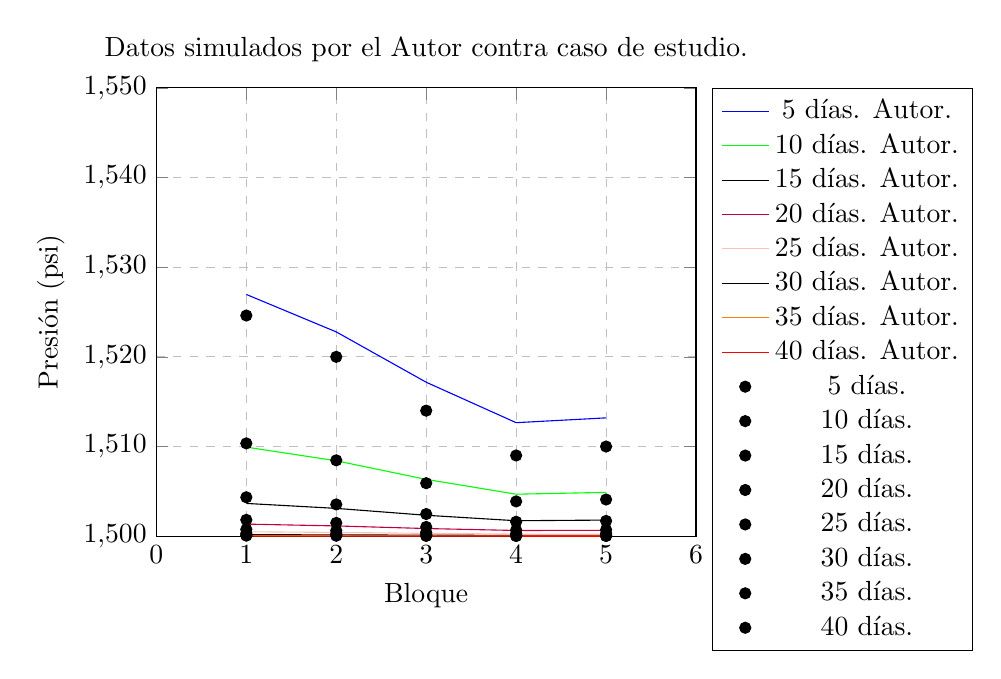
\begin{tikzpicture}
	\begin{axis}[
	title={Datos simulados por el Autor contra caso de estudio.},
	xlabel={Bloque},
	ylabel={Presión (psi)},
	xmin=0, xmax=6,
	ymin=1500, ymax=1550,
	legend pos=outer north east ,
	ymajorgrids=true,
	xmajorgrids=true,
	%semilogxaxis=true,
	grid style=dashed,
	]
	
	\addplot[color=blue]
	coordinates{
		(1,	1526.960064 )
		(2,	1522.7829696)
		(3,	1517.169999)
		(4,	1512.6593172)
		(5,	1513.1959578)
	};
	\addlegendentry{5 días. Autor.}
	
	\addplot[color=green]
	coordinates{
		(1,	1509.9326028)
		(2,	1508.4097038)
		(3,	1506.3356604)
		(4,	1504.6822272)
		(5,	1504.8852804)
	};
	\addlegendentry{10 días. Autor.}
	
	\addplot[color=black]
	coordinates{
		(1,	1503.6524574)
		(2,	1503.101313)
		(3,	1502.3326116)
		(4,	1501.723452)
		(5,	1501.795971)
	};
	\addlegendentry{15 días. Autor.}
	
	\addplot[color=purple]
	coordinates{
		(1,	1501.3463532)
		(2,	1501.1433)
		(3,	1500.853224)
		(4,	1500.635667)
		(5,	1500.6501708)
	};
	\addlegendentry{20 días. Autor.}
	
	\addplot[color=pink]
	coordinates{
		(1,	1500.490629)
		(2,	1500.41811)
		(3,	1500.3165834)
		(4,	1500.2295606)
		(5,	1500.2295606)
	};
	\addlegendentry{25 días. Autor.}
	
	
	\addplot[]
	coordinates{
		(1,	1500.1715454)
		(2,	1500.1425378)
		(3,	1500.1135302)
		(4,	1500.0845226)
		(5,	1500.0845226)
	};
	\addlegendentry{30 días. Autor.}
	
	\addplot[color=orange]
	coordinates{
		(1,	1500.055515)
		(2,	1500.0410112)
		(3,	1500.0265074)
		(4,	1500.0265074)
		(5,	1500.0265074)
	};
	\addlegendentry{35 días. Autor.}
	
	
	\addplot[red]
	coordinates{
		(1,	1500.0120036)
		(2,	1500.0120036)
		(3,	1500.0120036)
		(4,	1499.9974998)
		(5,	1499.9974998)
	};
	\addlegendentry{40 días. Autor.}
	
	
	\addplot[only marks]
	coordinates{
		(1,	1524.61)
		(2,	1520)
		(3,	1514)
		(4,	1509 )
		(5,	1510)
		
	};
	\addlegendentry{5 días. }
	
	\addplot[only marks]
	coordinates{
		(1,	1510.35)
		(2,	1508.46)
		(3,	1505.91)
		(4,	1503.88)
		(5,	1504.09)
		
	};
	\addlegendentry{10 días.}
	
	\addplot[only marks]
	coordinates{
		(1,	1504.34)
		(2,	1503.54)
		(3,	1502.47)
		(4,	1501.61)
		(5,	1501.7)
	};
	\addlegendentry{15 días. }
	
	\addplot[only marks]
	coordinates{
		(1,	1501.82)
		(2,	1501.48)
		(3,	1501.03)
		(4,	1500.68)
		(5,	1500.71)
	};
	\addlegendentry{20 días.}
	
	\addplot[only marks]
	coordinates{
		(1,	1500.76)
		(2,	1500.62)
		(3,	1500.43)
		(4,	1500.28)
		(5,	1500.3)
	};
	\addlegendentry{25 días.}
	
	
	\addplot[only marks]
	coordinates{
		(1,	1500.32)
		(2,	1500.26)
		(3,	1500.18)
		(4,	1500.12)
		(5,	1500.12)
	};
	\addlegendentry{30 días.}
	
	\addplot[only marks]
	coordinates{
		(1,	1500.13)
		(2,	1500.11)
		(3,	1500.08)
		(4,	1500.05)
		(5,	1500.05)
	};
	\addlegendentry{35 días.}
	
	
	\addplot[only marks]
	coordinates{
		(1	,1500.06)
		(2	,1500.05)
		(3	,1500.03)
		(4	,1500.02)
		(5	,1500.02)
	};
	\addlegendentry{40 días.}
	
	\end{axis}
	\end{tikzpicture}
	\caption{gg}
	\label{cora}
\end{figure}{}


\begin{figure}[h!]
	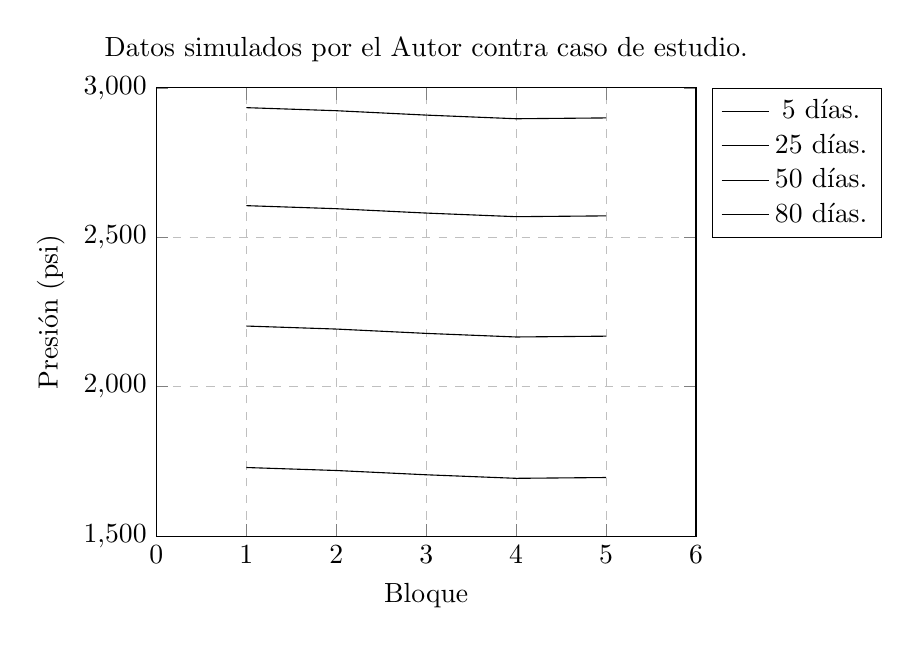
\begin{tikzpicture}
	\begin{axis}[
	title={Datos simulados por el Autor contra caso de estudio.},
	xlabel={Bloque},
	ylabel={Presión (psi)},
	xmin=0, xmax=6,
	ymin=1500, ymax=3000,
	legend pos=outer north east ,
	ymajorgrids=true,
	xmajorgrids=true,
	%semilogxaxis=true,
	grid style=dashed,
	]
	
	\addplot[]
	coordinates{
		(1,2933.8141602)	
		(2,2923.5889812)	
		(3,2908.882128)	
		(4,2896.698936)	
		(5,2899.4836656)
		
	};
	\addlegendentry{5 días.}
	
	\addplot[]
	coordinates{
		(1,2605.9267536)	
		(2,2595.745086)	
		(3,2581.1107518)	
		(4,2569.0000788)	
		(5,2571.741297)
		
	};
	\addlegendentry{25 días.}
	
	\addplot[]
	coordinates{
		(1,2203.1127162)	
		(2,2193.0180714)	
		(3,2178.5287752)	
		(4,2166.5196288)	
		(5,2169.2463432)
		
	};
	\addlegendentry{50 días.}
	
	\addplot[]
	coordinates{
		(1,1729.7812032)	
		(2,1719.8025888)	
		(3,1705.4728344)	
		(4,1693.6087260)
		(5,1696.3064328)
		
	};
	\addlegendentry{80 días.}
	\end{axis}
	\end{tikzpicture}
	\caption{gg izi}
	\label{siiiizas}
\end{figure}{}

\end{appendix}